\chapter{\textbf{Bit}maps for \textbf{D}isk \textbf{F}iltering (BitDF)}
\label{chp:algorithm}
\section{Problem Statement}
By analyzing some of the algorithms proposed in \secref{sec:rel_flocks} and their respective running times, we noticed
that most of the CPU cycles were spent by analyzing disks that will not generate flock patterns, due to the points no
being present in $\delta$ consecutive time slots. In all algorithms, disks generated in time slot $t_i$ are compared
with those generated in $t_{i+1}$ in order to check if an extension to a potential flock pattern is found. This
operation has $O(nm)$ complexity, with $n$ being the number of disks and $m$ the number of potential flocks from
previous time slots.  Additionally, for each comparison between a disk and a potential flock, an intersection operation
between them needs to be made.

Things get even worse in algorithms like BFE, where a new created disk $D$ is checked if it is either subset or a
duplicate of a previously found disk (as already mentioned in \secref{subsec:disk_discovery}). The running time of this
step can result in a $O(n^2)$ time complexity in the worst case (with $n$ being the number of disks generated by that
time slot) requiring an intersection operation between each pair of disks that are being compared. We can reduce
significantly that number of disks by only creating disks with points that can potentially form a flock, i.e. with
points that appears in the dataset for $\delta$ consecutive time slots. Such problem is well depicted in
\figref{fig:time_consumption}, where we can see that the disk and flock related operations can reach 99\% of the overall
processing time of the algorithm.

Consider the example depicted in Fig. \ref{fig:disks}, where we are looking for flocks with $\mu=4$ and $\delta=4$. As
we can see, in time slot $t_0$ our dataset reported points $p_1,p_2,p_3$ and $p_4$ and, due to the proximity between
them, disk $d_0$ was created enclosing all four points. In $t_1$ the same points were reported and again the regular
algorithm was able to create another disk $d_1$. However, in $t_2$, $p_3$ was not present and the disk $d_2$ only
contained three points, which is not enough to represent a flock pattern because the number of trajectories is less than
$\mu = 4$. Hence, we could avoid the creation of disks $d_0$ and $d_1$ if we would know in advance that $p_3$ was
missing in $t_2$, saving CPU cycles of disk comparisons in $t_0$ and $t_1$. We argue that when scaled to a dataset of
millions of records with real-time processing, that disk check for subsets and flock extension, in the regular
algorithms, will lead to severe degradation in performance. With that in mind, we can say with high confidence that
reducing the processing time spent with unnecessary disks that won't generate flock patterns, can dramatically reduce
the overall processing time of the algorithm.

\begin{figure}[h!]
    \centering
    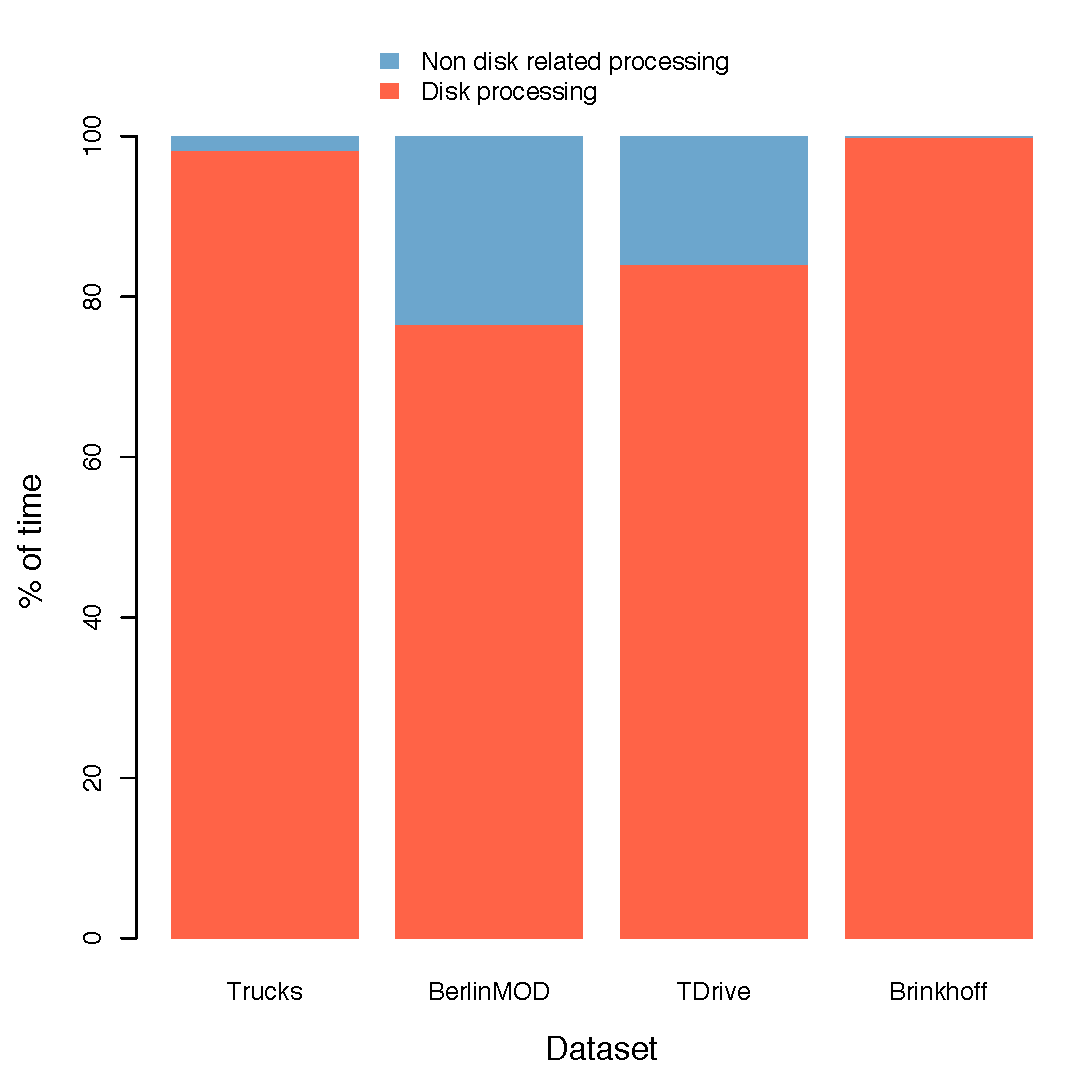
\includegraphics[width=0.7\linewidth]{images/timeConsumption.eps}
    \caption{Percentage of time spent between disk and flock processing tasks against other tasks in the algorithm}
    \label{fig:time_consumption}
\end{figure}

\begin{figure}[h!]
    \centering
    
\includegraphics[width=\linewidth]{images/disks_2.png}
    \caption{Sequence of disks in 4 consecutive time slots and the points that were clustered to them}
    \label{fig:disks}
\end{figure}

\section{Proposed Solution}
Our solution consist on using \textbf{Bit}maps for \textbf{D}isk \textbf{F}iltering (BitDF), based on the BFE algorithm.
BitDF splits the algorithm in two logical modules, namely GPS Stream Buffering (GSB) and Flock Processor (FP), and have
each of them keep track of the history of every $O_{id}$ in time.

Algorithm~\ref{alg:gpsb} shows that GSB will listen to the on-line GPS point stream, in the procedure
\textsc{ReceivePoints}, add each point to the \textit{pointBuffer} structure (which is a hash map of points by time
slot) and map each $O_{id}$ presence in time by calling \textsc{AddPointPresence}. When GSB has buffered $\delta$ time
slots (line 23) it will then send the points of $timeSlot - \delta$ to FP. After FP is done with its processing, GSB
will discard the first position of the presence maps, by calling \textsc{ShiftPresenceMaps}, and also discard the points
collected in $timeSlot - \delta$, which were already processed by FP. The flow continues indefinitely by buffering the
points from the next time slot $t_i$ and send the points from $t_{i - \delta}$ to FP for processing. It is worth noting
\textit{timeSlotSize} (line 21) refers to the time slot $\sigma$ introduced in \secref{sec:tech_data}.

Using Fig. \ref{fig:disks} as an example, we can see in Table \ref{tab:bitmaps} the state of the GSB bitmaps for each
$O_{id}$ after receiving the points in $t_3$. With those bitmaps, we can easily look up for a specific point occurrence
in time and check if that point in that specific time slot can potentially form a flock pattern or not. The bitmaps in
GSB will always refer to the "future" of a specific $O_{id}$.

In Algorithm~\ref{alg:fp_helpers} we start by first listing the procedures that will help the core procedure of FP (the
\textsc{Process}, in Algorithm~\ref{alg:fp}). It is also in Algorithm~\ref{alg:fp_helpers} that we list the most
important piece of this system that allows us to achieve such good optimizations, in both CPU cycles and memory
consumption, which is the \textsc{IsPointEligible} procedure. Such procedure is responsible to put together what
happened in the \textit{past} and what is going to happen in the \textit{future} for a given point $p$, in order to
decide whether $p$ can be part of a potential flock pattern or not. It does that by concatenating, for a given $O_{id}$,
the bitmap from FP with the bitmap from GSB (line 5 of Algorithm~\ref{alg:fp_helpers}) and searching for a sequence of
$\delta$ bits set to 1 (lines 6 to 15 of Algorithm~\ref{alg:fp_helpers}). That search is performed by combining AND and
XOR bitwise operations against the presence bitmap assembled in line 5 of Algorithm~\ref{alg:fp_helpers}. Whenever a
potential flock is found in a time slot $t_i$ and $p$ is part of it, we need to update its bitmap so when we process
points of time slot $t_{i+1}$ we have the correct bitmap representation of $p$ and that is where \textsc{MapPointFlock}
(line 20) comes to play. \textsc{MapPointFlock} does that by prepending 1 to $p$'s bitmap in FP module by perforing an
OR bitwise operation.

\begin{table}
    \renewcommand{\arraystretch}{1.3}
    \caption{Bitmaps in GSB after buffering four time slots}
    \label{tab:bitmaps}
    \centering
    \begin{tabular}{c|c}
        \hline
        $O_{id}$ &   Bitmap\\
        \hline
        \hline
        1        &   1111\\
        \hline
        2        &   0111\\
        \hline
        3        &   1011\\
        \hline
        4        &   1111\\
        \hline
    \end{tabular}
\end{table}

\begin{algorithm}
\caption{GPS Stream Buffering}
\label{alg:gpsb}
\begin{algorithmic}[1]
    \State $pointBuffer \gets map\{index, \{id, point[...]\}\}$
    \State $presenceMap \gets map\{id, bitmap\}$
    \State $lastTimeslot \gets -1$
    \State
    \Procedure{AddPointPresence}{$id$}
        \State $mask \gets \Call{ShiftLeft}{1, pointBuffer.size - 1}$
        \State $presence \gets \Call{BitOr}{presenceMap[id], mask}$
        \State $presenceMap[id] \gets presence$
    \EndProcedure
    \State
    \Procedure{ShiftPresenceMaps}{}
        \ForAll {$id \in \Call{Keys}{presenceMap}$}
            \State $shifted \gets \Call{ShiftRight}{presenceMap[id], 1}$
            \State $presenceMap[id] \gets shifted$
        \EndFor
    \EndProcedure
    \State
    \Procedure{ReceivePoints}{}
        \Loop
            \State $point \gets gpsPointStream.dequeue$
            \State $timeSlot \gets point.timestamp / timeSlotSize$
            \If{$timeSlot > lastTimeslot$}
                \If{$pointBuffer.size \ge \delta$}
                    \State \Call{Fp.Process}{pointBuffer.first}
                    \State \textbf{delete} $pointBuffer.first$
                    \State \Call{ShiftPresenceMaps}{}
                \EndIf
                \State $lastTimeslot \gets timeSlot$
            \EndIf
            \State $pointBuffer[timeSlot][point.id].append(point)$
            \State \Call{AddPointPresence}{$point.id$}
        \EndLoop
    \EndProcedure
\end{algorithmic}
\end{algorithm}

\begin{algorithm}
\caption{Flock Processor Helper Procedures}
\label{alg:fp_helpers}
\begin{algorithmic}[1]
    \State $buffered \gets 0$ \Comment max time span of the current flocks, max value is $\delta$
    \State $flockMap \gets map\{id, bitmap\}$
    \State
    \Procedure{IsPointEligible}{$id$}
        \State $presence \gets \Call{Concat}{presenceMap[id], flockMap[id]}$
        \State $eligibleMask \gets \Call{ShiftLeft}{1, \delta} - 1$
        \State $range \gets pointBuffer.size + buffered$
        \State $checks \gets \Call{Max}{1, range - \delta + 1}$
        \While{$checks > 0$}
            \State $tmp \gets \Call{BitAnd}{presence, eligibleMask}$
            \If{\Call{BitXor}{$tmp, eligibleMask$}}
                \State \Return $\textbf{\textit{true}}$
            \EndIf
            \State $checks \gets checks - 1$
            \State $eligibleMask \gets \Call{ShiftLeft}{eligibleMask, 1}$
        \EndWhile
        \State \Return $\textbf{\textit{false}}$
    \EndProcedure
    \State
    \Procedure{MapPointFlock}{$id$}
        \State $mask \gets \Call{ShiftLeft}{1, buffered}$
        \State $flockMap[id] \gets \Call{BitOr}{flockMap[id, mask}$
    \EndProcedure
    \State
    \Procedure{ShiftFlockMaps}{}
        \ForAll {$id \in \Call{Keys}{flockMap}$}
            \State $flockMap[id] \gets \Call{ShiftRight}{flockMap[id], 1}$
        \EndFor
    \EndProcedure
    \State
    \Procedure{StoreDiskIfEligible}{$diskSet, d$}
        \If{$\Call{Count}{d} \ge \mu \enspace \textbf{and} \enspace \textbf{not} \enspace \Call{SubSet}{d}$}
            \State \Call{AddDisk}{$diskSet, d$}
        \Else
            \State \textbf{delete} $d$
        \EndIf
    \EndProcedure
\end{algorithmic}
\end{algorithm}

\begin{algorithm}
\caption{Flock Processor Process Procedure}
\label{alg:fp}
\begin{algorithmic}[1]
    \Procedure{Process}{$pointMap\{id, point[...]\}, timeslot$}
        \State $D \gets \emptyset$
        \State $cells \gets \Call{BuildGrid}{pointMap}$
        \If{$buffered \ge \delta$}
            \State \Call{ShiftFlockMaps}{}
            \State $buffered \gets buffered - 1$
        \EndIf
        \ForAll{$c_{x, y} \in cells$}
            \State $cellRange \gets [c_{x - 1, y - 1}...c_{x + 1, y+ 1}]$
            \ForAll{$p1 \in c_{x, y}$}
                \ForAll{$p2 \in cellRange$}
                    \If{$d(p1, p2) \le \epsilon$}
                        \State $d1, d2 \gets \Call{CreateDisks}{p1, p2}$
                        \ForAll{$p \in cellRange$}
                            \State $added \gets \textbf{false}$
                            \If{$\Call{InDisk}{d1, p} \enspace \textbf{and} \enspace \Call{IsPointEligible}{p}$}
                                \State $\Call{Add(d1, p)}$
                                \State $added \gets \textbf{true}$
                            \EndIf
                            \If{$\Call{InDisk}{d2, p} \enspace \textbf{and} \enspace \Call{IsPointEligible}{p}$}
                                \State $\Call{Add(d2, p)}$
                                \State $added \gets \textbf{true}$
                            \EndIf
                            \If{$added = \textbf{true}$}
                                \State $\Call{MapPointFlock}{p.id}$
                            \EndIf
                        \EndFor
                        \State \Call{StoreDiskIfEligible}{$D, d1$}
                        \State \Call{StoreDiskIfEligible}{$D, d2$}
                    \EndIf
                \EndFor
            \EndFor
        \EndFor
        \State $buffered \gets buffered + 1$
    \EndProcedure
\end{algorithmic}
\end{algorithm}

\figref{fig:flow} shows how GSB and FP will interact in a scenario where $\mu = 3$ and $\delta = 3$. First, GSB will
buffer points and build the bitmaps for each of them until it finishes receiving points from $t_2$. At that time, points
$p_1$, $p_2$, $p_3$ and $p_4$ will have the bitmaps as stated in the GSB module, under the bitmap column for time slot
$t_2$. Then, the next step will be to call \textsc{Process} (Algorithm~\ref{alg:fp}) of FP with points from time slot
$t_0$, which will be all the four points (as we can see in the bitmaps in GSB, all points were present in time slot
$t_0$). Since FP has not processed any points so far, its bitmaps structures are empty and the concatenation of the
bitmaps from both modules will end up as being the same value as in GSB. By the end of $t_0$ processing, one disk is
generated, containing only $p_1$, $p_2$ and $p_4$, having $p_3$ being ignored due to its bitmap telling that it cannot
form a flock starting from $t_0$. The flow then continues repeating the same steps that we mentioned above, until a
flock contaning points $p_1$, $p_2$ and $p_4$ is found.

\begin{figure}
    \centering
    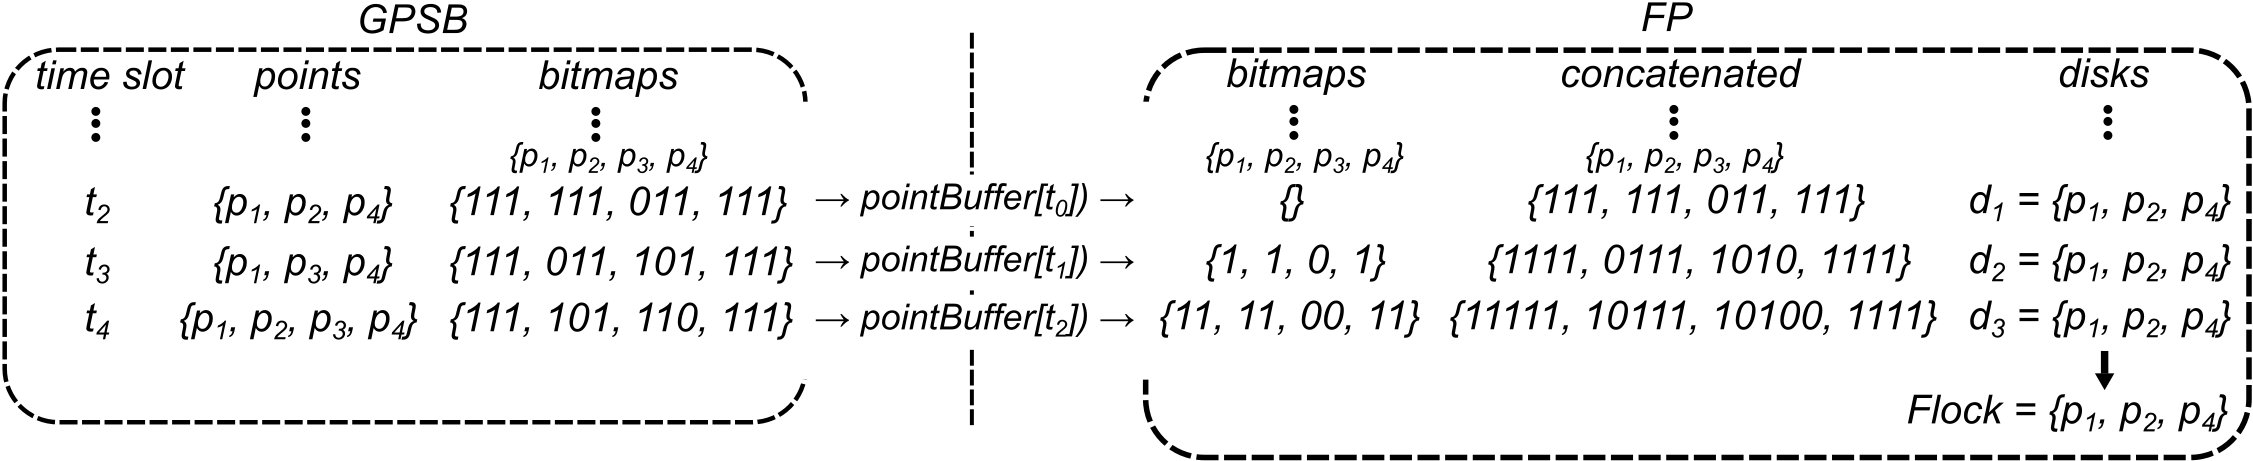
\includegraphics[width=\linewidth]{images/flow.png}
    \caption{Find flock without creating unnecessary disks. Bitmap buffers from both GSB and FP, in an example where
        $\delta = 3$}
    \label{fig:flow}
\end{figure}
